%%%%%%%%%%%%%%%%%%%%%%%%%%%%%%%%%%%%%%%%%%%%%%%%%%%%%%%%%%%%%%%%%%%%%%%%%%%%
% AGUtmpl.tex: this template file is for articles formatted with LaTeX2e,
% Modified November 2013
%
% This template includes commands and instructions
% given in the order necessary to produce a final output that will
% satisfy AGU requirements.
%
% PLEASE DO NOT USE YOUR OWN MACROS
% DO NOT USE \newcommand, \renewcommand, or \def.
%
% FOR FIGURES, DO NOT USE \psfrag
%
%%%%%%%%%%%%%%%%%%%%%%%%%%%%%%%%%%%%%%%%%%%%%%%%%%%%%%%%%%%%%%%%%%%%%%%%%%%%
%
% All questions should be e-mailed to latex@agu.org.
%
%%%%%%%%%%%%%%%%%%%%%%%%%%%%%%%%%%%%%%%%%%%%%%%%%%%%%%%%%%%%%%%%%%%%%%%%%%%%
%
% Step 1: Set the \documentclass
%
% There are two options for article format: two column (default)
% and draft.
%
% PLEASE USE THE DRAFT OPTION TO SUBMIT YOUR PAPERS.
% The draft option produces double spaced output.
%
% Choose the journal abbreviation for the journal you are
% submitting to:

% jgrga JOURNAL OF GEOPHYSICAL RESEARCH
% gbc   GLOBAL BIOCHEMICAL CYCLES
% grl   GEOPHYSICAL RESEARCH LETTERS
% pal   PALEOCEANOGRAPHY
% ras   RADIO SCIENCE
% rog   REVIEWS OF GEOPHYSICS
% tec   TECTONICS
% wrr   WATER RESOURCES RESEARCH
% gc    GEOCHEMISTRY, GEOPHYSICS, GEOSYSTEMS
% sw    SPACE WEATHER
% ms    JAMES
% ef    EARTH'S FUTURE
%
%
%
% (If you are submitting to a journal other than jgrga,
% substitute the initials of the journal for "jgrga" below.)

\documentclass[draft,jgrga]{agutexSI2018}
%\documentclass{article}


%%%%%%%%%%%%%%%%%%%%%%%%%%%%%%%%%%%%%%%%%%%%%%%%%%%%%%%%%%%%%%%%%%%%%%%%%
%
%  SUPPORTING INFORMATION TEMPLATE
%
%% ------------------------------------------------------------------------ %%
%
%
%Please use this template when formatting and submitting your Supporting Information.

%This template serves as both a “table of contents” for the supporting information for your article and as a summary of files.
%
%
%OVERVIEW
%
%Please note that all supporting information will be peer reviewed with your manuscript.
%In general, the purpose of the supporting information is to enable authors to provide and archive auxiliary information such as data %tables, method information, figures, video, or computer software, in digital formats so that other scientists can use it.
%The key criteria are that the data:
% 1. supplement the main scientific conclusions of the paper but are not essential to the conclusions (with the exception of
%    including %data so the experiment can be reproducible);
% 2. are likely to be usable or used by other scientists working in the field;
% 3. are described with sufficient precision that other scientists can understand them, and
% 4. are not exe files.
%
%USING THIS TEMPLATE
%
%All Supporting text and figures should be included in this document. Insert supporting information content into each appropriate section of the template. %Figures and tables should appear above each caption.  To add additional captions, simply copy and paste each sample caption as needed.

%Tables may be included, but can also be uploaded separately, especially if they are larger than 1 page, or if necessary for retaining table formatting. Data sets, large tables, movie files, and audio files should be uploaded separately, following AGU naming conventions. Include their captions in this document and list the file name with the caption. You will be prompted to upload these files on the Upload Files tab during the submission process, using file type “Supporting Information (SI)”

%IMPORTANT NOTE ON FIGURES AND TABLES
% Placeholders for figures and tables appear after the \end{article} command, after references.
% DO NOT USE \psfrag or \subfigure commands.
%
%  Uncomment the following command to include .eps files
 \usepackage{amsmath} 
 \usepackage{graphicx}
%
%  Uncomment the following command to allow illustrations to print
%   when using Draft:
 \setkeys{Gin}{draft=false}
%
% Substitute one of the following for [dvips] above
% if you are using a different driver program and want to
% proof your illustrations on your machine:
%
% [xdvi], [dvipdf], [dvipsone], [dviwindo], [emtex], [dviwin],
% [pctexps],  [pctexwin],  [pctexhp],  [pctex32], [truetex], [tcidvi],
% [oztex], [textures]
%
%
%% ------------------------------------------------------------------------ %%
%
%  ENTER PREAMBLE
%
%% ------------------------------------------------------------------------ %%

% Author names in capital letters:
%\authorrunninghead{LILENSTEN ET AL.}

% Shorter version of title entered in capital letters:
%\titlerunninghead{AURORAL ANGLE OF LINEAR POLARISATION}

%Corresponding author mailing address and e-mail address:
%\authoraddr{Corresponding author: J. Lilensten,
%UJF-Grenoble 1 / CNRS-INSU, Institut de Plan\'etologie et d'Astrophysique de Grenoble (IPAG), UMR 5274, Grenoble, F-38041, France
%(jean.lilensten@univ-grenoble-alpes.fr)}

\begin{document}

%% ------------------------------------------------------------------------ %%
%
%  TITLE
%
%% ------------------------------------------------------------------------ %%

%\includegraphics{agu_pubart-white_reduced.eps}


\title{Supporting Information for "The thermospheric auroral red line Angle of Linear Polarisation"}
\authors{J. Lilensten,\altaffilmark{1}
Mathieu Barth\'elemy ,\altaffilmark{1} G. Besson,\altaffilmark{2}
Herv\'e Lamy, \altaffilmark{3} Magnar G. Johnsen, \altaffilmark{4}, and J\o ran Moen\altaffilmark{5}}

\altaffiltext{1}{UJF-Grenoble 1 / CNRS-INSU, Institut de Plan\'etologie et d'Astrophysique de Grenoble (IPAG), UMR 5274, Grenoble, F-38041, France}

\altaffiltext{2}{Institut Fourier, Universit\'e de Grenoble, France}

\altaffiltext{3}{Belgian Institute for Space Aeronomy, Ringlaan-3-Avenue Circulaire, B-1180 Brussels, Belgium}

\altaffiltext{4}{Troms\o\ Geophysical Observatory University of Troms\o, Norway}

\altaffiltext{5}{Department of Physics, University of Oslo, P.O. Box 1048, N-0316 Blindern, Oslo, Norway}


\begin{article}

\noindent\textbf{Contents of this file}
\begin{enumerate}
\item Text S1 to S5
\item Figures S1 to S10
\end{enumerate}

\section{Introduction}
Computing the apparent angle of the magnetic field as seen by the polarimeter in any direction is a classical spherical geometry problem. However, it is difficult to find the development in geophysical articles or textbooks. Therefore, we chose to provide it here. It is not something new, reason to write it as an appendix.
\section{Geographical coordinates}
The geography is plotted in Figure \ref{geography_1}. The SPP is located at a point $A$ characterized by a latitude $\Phi_{A}$ and a longitude $\Psi_{A}$. It looks at the polarisation with an elevation $\epsilon$ and an azimuth $\alpha$. The elevation is the angle with the plan which is tangent to the sphere in $A$, $\epsilon = 0^\circ$ when pointing at the horizon and$\epsilon = 90^\circ$ when pointing at the zenith. The azimuth is the angle with the meridian in $A$. It is taken equal to zero pointing North, to $90^\circ$ East, $180^\circ$ South and $270^\circ$ West. \\

In \citep{Lilensten_pola2015}, we have shown that the theoretical polarisation equals the observations at the altitude at which the red line emission maximizes. Let us call $h$ this altitude. In the above comparison, following  \citep{Lilensten_pola2015}, $h = 220\ km$. We call $H$ the point where the line of sight is at an altitude $h$. If $O$ is the center of the Earth, the axis $\bar{OH}$ intersects the surface of the Earth at a point $P$ of latitude $\Phi_{H}$ and longitude $\Psi_{H}$. The line of sight $\overrightarrow{AH}$ has a norm $\vert AH \vert$ and is carried by the unit vector $\overrightarrow{u}$.\\
The frame of reference $\mathcal{R}_O$ at $O$ is as follows: Axis $x$ is at zeroth longitude and latitude. Axis $y$ is horizontal and points positively toward longitude 90. Axis $z$ is vertical and points positively toward the north pole.
The frame of reference $\mathcal{R}_A$ at $A$ is as follows: Axis $x$ is the altitude, positive upward. Axis $y$ points positively toward the east in the plan tangent to the surface in $A$. Axis $z$ points positively toward the north in the same plan. Let us compute $\Phi_{H}$ and $\Psi_{H}$. In the following, $R_T^A$ is the radius of the Earth in $A$.

\section{First step: $A$ at the equator}
We now consider that $A$ is located at the equator such as shown in Figure \ref{geography_2}, along the zeroth meridian. The reference frame in $A$ is the same as the reference frame in $O$, the center of the Earth, translated by a distance $R_t^A$ along the x axis. We call \{X,Y,Z\} the absolute frame centered around $O$. A magnification of the geometry around a is plotted in figure \ref{geometrie}.

\begin{equation}
\left\{ \begin{array}{cc}
\Phi_{A} &=\ 0 \\
\Psi_{A} &=\ 0 
\end{array} \right.
\label{coord_eq}
\end{equation}

Expressed in $\mathcal{R}_A$, the projection of $\overrightarrow{u}$ in the horizontal plane is (Figure \ref{geography_2}):

\begin{equation}
\left\{ \begin{array}{cc}
u_y &=\ \sin(\alpha_{AH}) \\
u_z &=\ \cos(\alpha_{AH}) 
\end{array} \right.
\label{vect_eq}
\end{equation}

With the choice of the azimuth oriented positively clockwise. Taking the elevation into account, one gets in $\mathcal{R}_A$:

\begin{equation}
\left\{ \begin{array}{cll}
u_x &=\ \sin(\epsilon_{AH}) & \textrm{altitude} \\
u_y &=\ \sin(\alpha_{AH})\cos(\epsilon_{AH})& \textrm{estward} \\
u_z &=\ \cos(\alpha_{AH}) \cos(\epsilon_{AH})& \textrm{northward}
\end{array} \right.
\label{vect_eq_proj}
\end{equation}


The vector that links the center of the Earth $O$ to the observed point $H$ is $\overrightarrow{OH}=\overrightarrow{OA} + \vert AH \vert \ \overrightarrow{u}$. We can develop on the three axis \{X, Y, Z\} of $\mathcal{R}_O$:

\begin{equation}
\overrightarrow{OH}=\left\{ \begin{array}{c}
R_T^A+\vert AH \vert\sin(\epsilon_{AH})\\
-\vert AH \vert\sin(\alpha_{AH})\cos(\epsilon_{AH}) \\
-\vert AH \vert\cos(\alpha_{AH}) \cos(\epsilon_{AH})
\end{array} \right.
\end{equation}

The norm of $\overrightarrow{OH}$ is $\vert OH \vert = \sqrt{OH_x^2+OH_y^2+OH_z^2}$, which gives:

\begin{equation}
\label{OH1}
\vert OH \vert = \sqrt{(R_T^A)^2+\vert AH \vert^2+2R_T^A \vert AH \vert \sin(\epsilon_{AH}})
\end{equation}


The height of the observation point H above the Earth is $h = \vert PH \vert$, which we take equal to 220 km. This value is the difference $\vert OH \vert - \vert OP \vert$. We suppose that the radius of the Earth is the same for $\vert OA \vert$ and $\vert OP \vert$ so that:

\begin{equation}
\label{OH2}
\vert OH \vert = h + R_T^A 
%= \sqrt{(R_T^A)^2+\vert AH \vert^2+2R_T^A \vert AH \vert \sin(\epsilon_{AH}})
\end{equation}

from equations \ref{OH1} and \ref{OH2} we easily get the value of $\vert AH \vert$ through:

\begin{equation}
\vert AH \vert^2 + 2\vert AH \vert\ R_T^A\sin(\epsilon_{AH}) -2 R_T^A h - h^2 = 0
\end{equation}

which gives:
\begin{equation}
\label{normAH}
\vert AH \vert = {R_T^A}^2\sin(\epsilon)^2 + \sqrt{{R_T^A}^2 \sin(\epsilon)^2 + 2hR_T^A + h^2}
\end{equation}

%The altitude component $OP_x(eq)$ is not equal to the radius of the Earth $R_T^A$ since it is a projection on the altitude axis going through A. Only if $\epsilon_{AH}=\frac{\pi}{2}$, i.e. one looks to the zenith, one retrieves that $\vert OP(eq) \vert = R_T^A$ and $\vert PH \vert = \vert AH \vert$. This of course is checked in the code solving this set of equations.\\
From equations \ref{vect_eq_proj} and \ref{normAH}, one deduces the vector $\overrightarrow{AH}$:

\begin{equation}
\overrightarrow{AH}=\vert AH \vert\ \overrightarrow{u} 
\label{vectAH}.
\end{equation}

\section{Second step: At any location}
The geometry of the problem is displayed in Figure \ref{geography_1}. The SPP may be positioned anywhere on Earth, and this complicate significantly the geometry. The first step is to find a way to express every vector in the same reference frame. 

Let us first express $\overrightarrow{u_A}$, the unit vector of our line of sight in $\mathcal{R}_O$. The transformation matrix to pass from the reference frame $\mathcal{R}_A$ at point $A$ to $\mathcal{R}_O$ at point $O$ is:

\begin{equation}
\label{rot_matrix}
R_{A \rightarrow O} = \begin{bmatrix}
   \cos(\Phi_A)cos(\psi_A) & -\sin(\psi_A)	& -\sin(\Phi_A)\cos(\psi_A) \\
   \cos(\Phi_A)sin(\psi_A) & \cos(\psi_A) 	& -\sin(\Phi_A)\sin(\psi_A) \\
   \sin(\Phi_A) 		 	  & 0			& \cos(\Phi_A)			  \\
   \end{bmatrix}
\end{equation}

And its inverse, $R_{O \rightarrow A}$, to pass from $\mathcal{R}_O$ to $\mathcal{R}_A$ is the transposed matrix of $R_{A \rightarrow O}$.
This will allow us to easily express all our vectors in one reference frame. For example, $\overrightarrow{u_A}$ can be expressed as follows in $\mathcal{R}_0$:

\begin{equation}
\overrightarrow{u_O} = R_{A \rightarrow O}. \overrightarrow{u_A}
\end{equation}

Using again the fact that $\overrightarrow{OH}=\overrightarrow{OA} + \vert AH \vert \ \overrightarrow{u}$, we can develop on the three axis \{X, Y, Z\} of $\mathcal{R}_O$:

\begin{equation}
\overrightarrow{OH}=
R_T^A \left( \begin{array}{c}
\cos(\Phi_A)\cos(\Psi_A)\\
\cos(\Phi_A)\sin(\Psi_A)\\
\sin(\Phi_A)
\end{array} \right)
+
\vert AH \vert \overrightarrow{u_O}
\end{equation}


From the vector $\overrightarrow{OH}$ , we can easily deduce the latitude $\Phi_H $ and the longitude $\Psi_H$ of the point H. Its elevation is still taken to be 220 km (see Figure \ref{geometrie}).

\begin{equation}
\label{latP}
\left\{ \begin{array}{cc}
\sin(\Phi_{H}  ) &=\ \frac{OH_z  }{\vert OH   \vert} \\
\cos(\Phi_{H}  ) &=\ \frac{\sqrt{OH_x^2  +OH_y^2  }}{\vert OH   \vert} 
\end{array} \right.
\end{equation}

\begin{equation}
\label{longH1}
\left\{ \begin{array}{cc}
\sin(\Psi_{H} ) &=\  \frac{OH_y }{\sqrt{OH_x^2 +OH_y^2 }} \\
\cos(\Psi_{H} ) &=\  \frac{OH_x }{\sqrt{OH_x^2 +OH_y^2 }}  
\end{array} \right.
\end{equation}

The results above Ny-\AA lesund are shown in Figure \ref{angtest}.

\section{Apparent angle of observation}
We use IGRF \citep{Olsen_2000} to get the magnetic field $B_H(H)$ at the observed point of coordinates $(latitude\ =\Phi_{H}\ longitude\ =\Psi_{H}\ heigh=220\ km$). The configuration is shown in Figure \ref{ChampMagn}. The next question to solve is that of the apparent angle of the magnetic field in $H$ seen from $A$.\\
IGRF provides the three coordinates of the magnetic field \{$B_x$,$B_y$,$B_y$\} in the frame of $H$, characterized by three axis  \{$x_H$,$y_H$,$z_H$\}. It is necessary to rotate these values in the reference frame of $A$, characterized by  \{$x_A$,$y_A$,$z_A$\}. This is illustrated in Figure \ref{rotation}.
   
The first rotation expresses the magnetic field $B_H$ in $\mathcal{R}_O$ using equation \ref{rot_matrix}:
   
\begin{equation}
\overrightarrow{B_O} = R_{H \rightarrow O}.\overrightarrow{B_H}
\end{equation}

The second rotation brings the field in $\mathcal{R}_A$:
   
\begin{equation}
\begin{array}{cl}
\overrightarrow{B_A} &=\ R_{O \rightarrow A}.\overrightarrow{B_O} \\
					&=\ R_{O \rightarrow A}.R_{H \rightarrow O}.\overrightarrow{B_H}
\end{array}
\end{equation}


Computing the magnetic angle seen by the SPP is performed through a last set of rotations that brings the magnetic field $\overrightarrow{B_A(H)}$ in the frame of the polarimeter $\mathcal{R}_{SPP} = \{x_{SPP},y_{SPP},z_{SPP}\}$. The rotations are illustrated in Figure \ref{lastrot}. 
The rotation matrix is:

\begin{equation}
R_{SPP \rightarrow A}=
\begin{pmatrix}
\sin(\epsilon) & 0 & \cos(\epsilon) \\
\cos(\epsilon)\sin(\alpha) & -\cos(\alpha) & -\sin(\epsilon)\sin(\alpha) \\
\cos(\epsilon)\cos(\alpha)  & \sin(\alpha) & -\sin(\epsilon)\cos(\alpha) 
\end{pmatrix}
\end{equation}

And again, its inverse matrix to pass from the reference frame of A to the reference frame of SPP is its transposed matrix $R_{A \rightarrow SPP}$.

So that we can now write the vector of the magnetic field  $\overrightarrow{B_{SPP}(H)}$ as seen by the polarimeter:

\begin{equation}
\begin{array}{cl}

\overrightarrow{B_{SPP}} &=\ R_{A \rightarrow SPP} \overrightarrow{B_A(H)} \\
						&=\ R_{A \rightarrow SPP}.R_{O \rightarrow A}.R_{H \rightarrow O}.\overrightarrow{B_H(H)}
						
\end{array}
\end{equation}

The apparent angle of the magnetic field is $\eta$ defined simply by:

\begin{equation}
\label{longP2}
\left\{ \begin{array}{cc}
\cos(\eta) &=\  \frac{B_y(SPP)}{\sqrt{B_z^2(SPP)+B_y^2(SPP)}} \\
\sin(\eta) &=\  \frac{B_z(SPP)}{\sqrt{B_z^2(SPP)+B_y^2(SPP)}}  
\end{array} \right.
\end{equation}

Figure \ref{fig_eta} shows this angle as a function of the elevation in four geographic directions. Obviously, at an elevation of $90^\circ$, all the values converge since this is a zenith pointing.   \\
The wriggle at $85^\circ$ in the south and north azimuth is due to the shape of the magnetic field, and more exactly to the eastward component of the magnetic field. As seen in Figure \ref{wriggle}, this component turns from positive to negative for the northern azimuth above $86^\circ$ while it turns from negative to positive for the southern azimuth.

\section{Angle between the line of sight and the magnetic field in P versus the SPP elevation.}
In \cite{Lilensten_pola2015}, we computed the theoretical Degree of Linear Polarisation. This value depends on the the angle $\Theta$ between the line of sight $\vert AH \vert$ (equation \ref{vectAH}) and the local magnetic field line in H $\overrightarrow{B_H(H)}$ (equation \ref{B_A}). It is simply computed through:

\begin{equation}
\cos(\Theta)= \frac{\overrightarrow{AH}.\overrightarrow{B_A(H)}}{\vert AH \vert\vert B_A(H)\vert}
\end{equation}

In Figure \ref{fig_theta}, we show this angle. Because we are still relatively low at 220 km, the magnetic field lines are almost vertical straight lines. At an elevation of $30^\circ$ as in the present study, this angle is $67.2^\circ$ in the west azimuth and $52^\circ$ in the Eastward direction. North and south directions give roughly the same angle of $60^\circ$. This contradicts our first articles \citep{Lilensten_decouverte} where we mentioned that our north pointing was close to a right angle. The error was due to the fact that we had used a simplified geometry. This has a effect on the published values of the DoLP (out of the scope of this article). The measured $DoLP_{obs}$ is a projection of the absolute value $DoLP_{abs}$ on the line of sight. We have therefore:

\begin{equation}
DoLP_{abs} = DoLP_{obs} \sin\Theta  
\label{sintheta}
\end{equation}

In our case, $\sin\Theta = 0.92$, introducing an error of 8\% when a right angle is considered.

\end{article}
\end{document}


%% ------------------------------------------------------------------------ %%
%%  REFERENCE LIST AND TEXT CITATIONS
%
% Either type in your references using
% \begin{thebibliography}{}
% \bibitem{}
% Text
% \end{thebibliography}
%
% Or,
%
% If you use BiBTeX for your references, please use the agufull08.bst file (available at % ftp://ftp.agu.org/journals/latex/journals/Manuscript-Preparation/) to produce your .bbl
% file and copy the contents into your paper here.
%
% Follow these steps:
% 1. Run LaTeX on your LaTeX file.
%
% 2. Make sure the bibliography style appears as \bibliographystyle{agufull08}. Run BiBTeX on your LaTeX
% file.
%
% 3. Open the new .bbl file containing the reference list and
%   copy all the contents into your LaTeX file here.
%
% 4. Comment out the old \bibliographystyle and \bibliography commands.
%
% 5. Run LaTeX on your new file before submitting.
%
% AGU does not want a .bib or a .bbl file. Please copy in the contents of your .bbl file here.

\begin{thebibliography}{12}
jeanj\providecommand{\natexlab}[1]{#1}
\expandafter\ifx\csname urlstyle\endcsname\relax
  \providecommand{\doi}[1]{doi:\discretionary{}{}{}#1}\else
  \providecommand{\doi}{doi:\discretionary{}{}{}\begingroup
  \urlstyle{rm}\Url}\fi

\bibitem[{\textit{{Lilensten} et~al.}(2008)\textit{{Lilensten}, {Moen},
  {Barth{\'e}lemy}, {Thissen}, {Simon}, {Lorentzen}, {Dutuit}, {Amblard}, and
  {Sigernes}}}]{Lilensten_decouverte}
{Lilensten}, J., J.~{Moen}, M.~{Barth{\'e}lemy}, R.~{Thissen}, C.~{Simon},
  D.~A. {Lorentzen}, O.~{Dutuit}, P.~O. {Amblard}, and F.~{Sigernes} (2008),
  {Polarisation in aurorae: A new dimension for space environments studies},
  \textit{Geophysical Research Letters}, \textit{35}, 8804,
  \doi{10.1029/2007GL033006}.

\bibitem[{\textit{{Lilensten} et~al.}(2015)\textit{{Lilensten}, {Bommier},
  {Barth{\'e}lemy}, {Bernard}, {Lamy}, {Moen}, {Johnsen}, {L\o vhaug}, and
  {Pitout}}}]{Lilensten_pola2015}
{Lilensten}, J., V.~{Bommier}, M.~{Barth{\'e}lemy}, D.~{Bernard}, H.~{Lamy},
  J.~{Moen}, M.~{Johnsen}, U.~{L\o vhaug}, and F.~{Pitout} (2015), {The auroral red line polarisation: modelling and measurements},
  \textit{Journal of Space Weather and Space Climate},
  \textit{5}, A26, \doi{10.1051/swsc/2015027}.
  
  \bibitem[{\textit{{Olsen} et~al.}(2000)\textit{{Olsen}, {Sabaka}, and
  {T{\o}ffner-Clausen}}}]{Olsen_2000}
{Olsen}, N., T.~J. {Sabaka}, and L.~{T{\o}ffner-Clausen} (2000), {Determination
  of the IGRF 2000 model}, \textit{Earth, Planets, and Space}, \textit{52},
  1175--1182, \doi{10.1186/BF03352349}.

\end{thebibliography}

%Reference citation examples:

%...as shown by \textit{Kilby} [2008].
%...as shown by {\textit  {Lewin}} [1976], {\textit  {Carson}} [1986], {\textit  {Bartholdy and Billi}} [2002], and {\textit  {Rinaldi}} [2003].
%...has been shown [\textit{Kilby et al.}, 2008].
%...has been shown [{\textit  {Lewin}}, 1976; {\textit  {Carson}}, 1986; {\textit  {Bartholdy and Billi}}, 2002; {\textit  {Rinaldi}}, 2003].
%...has been shown [e.g., {\textit  {Lewin}}, 1976; {\textit  {Carson}}, 1986; {\textit  {Bartholdy and Billi}}, 2002; {\textit  {Rinaldi}}, 2003].

%...as shown by \citet{jskilby}.
%...as shown by \citet{lewin76}, \citet{carson86}, \citet{bartoldy02}, and \citet{rinaldi03}.
%...has been shown \citep{jskilbye}.
%...has been shown \citep{lewin76,carson86,bartoldy02,rinaldi03}.
%...has been shown \citep [e.g.,][]{lewin76,carson86,bartoldy02,rinaldi03}.
%
% Please use ONLY \citet and \citep for reference citations.
% DO NOT use other cite commands (e.g., \cite, \citeyear, \nocite, \citealp, etc.).

%% ------------------------------------------------------------------------ %%
%
%  END ARTICLE
%
%% ------------------------------------------------------------------------ %%
\end{article}
\clearpage

\newpage
  \begin{figure}
   \setfigurenum{S1}
   \noindent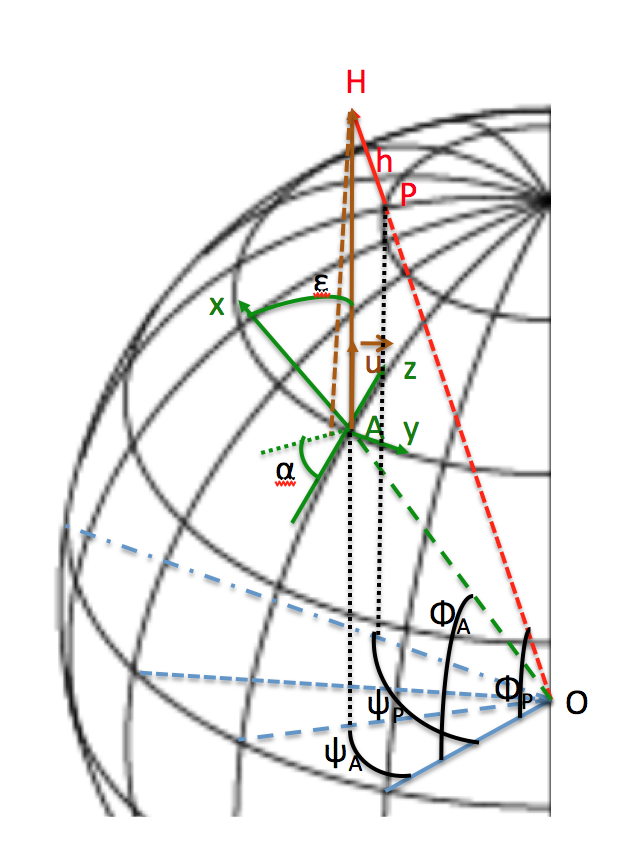
\includegraphics[width=9cm]{figures/Reel_scan.pdf}
   \caption{Geometry of the problem} 
   \label{geography_1}
   \end{figure}

  \begin{figure}
   \setfigurenum{S2}
   \noindent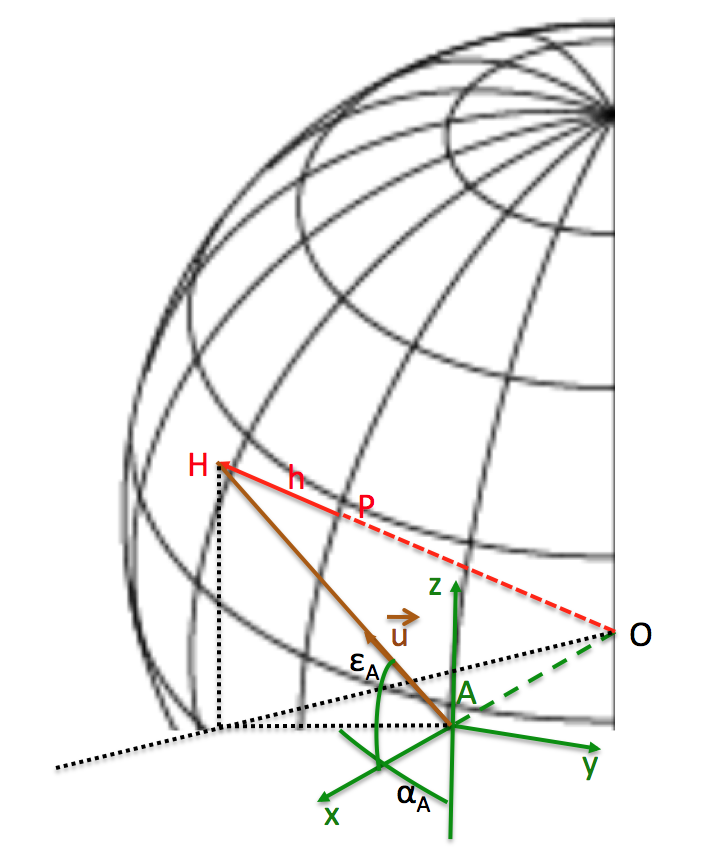
\includegraphics[width=9cm]{figures/Equateur_avec_2reperes.pdf}
   \caption{Geometry of the problem when the instrument is at the equator.} 
   \label{geography_2}
   \end{figure}
   
  \begin{figure}
   \setfigurenum{S3}
   \noindent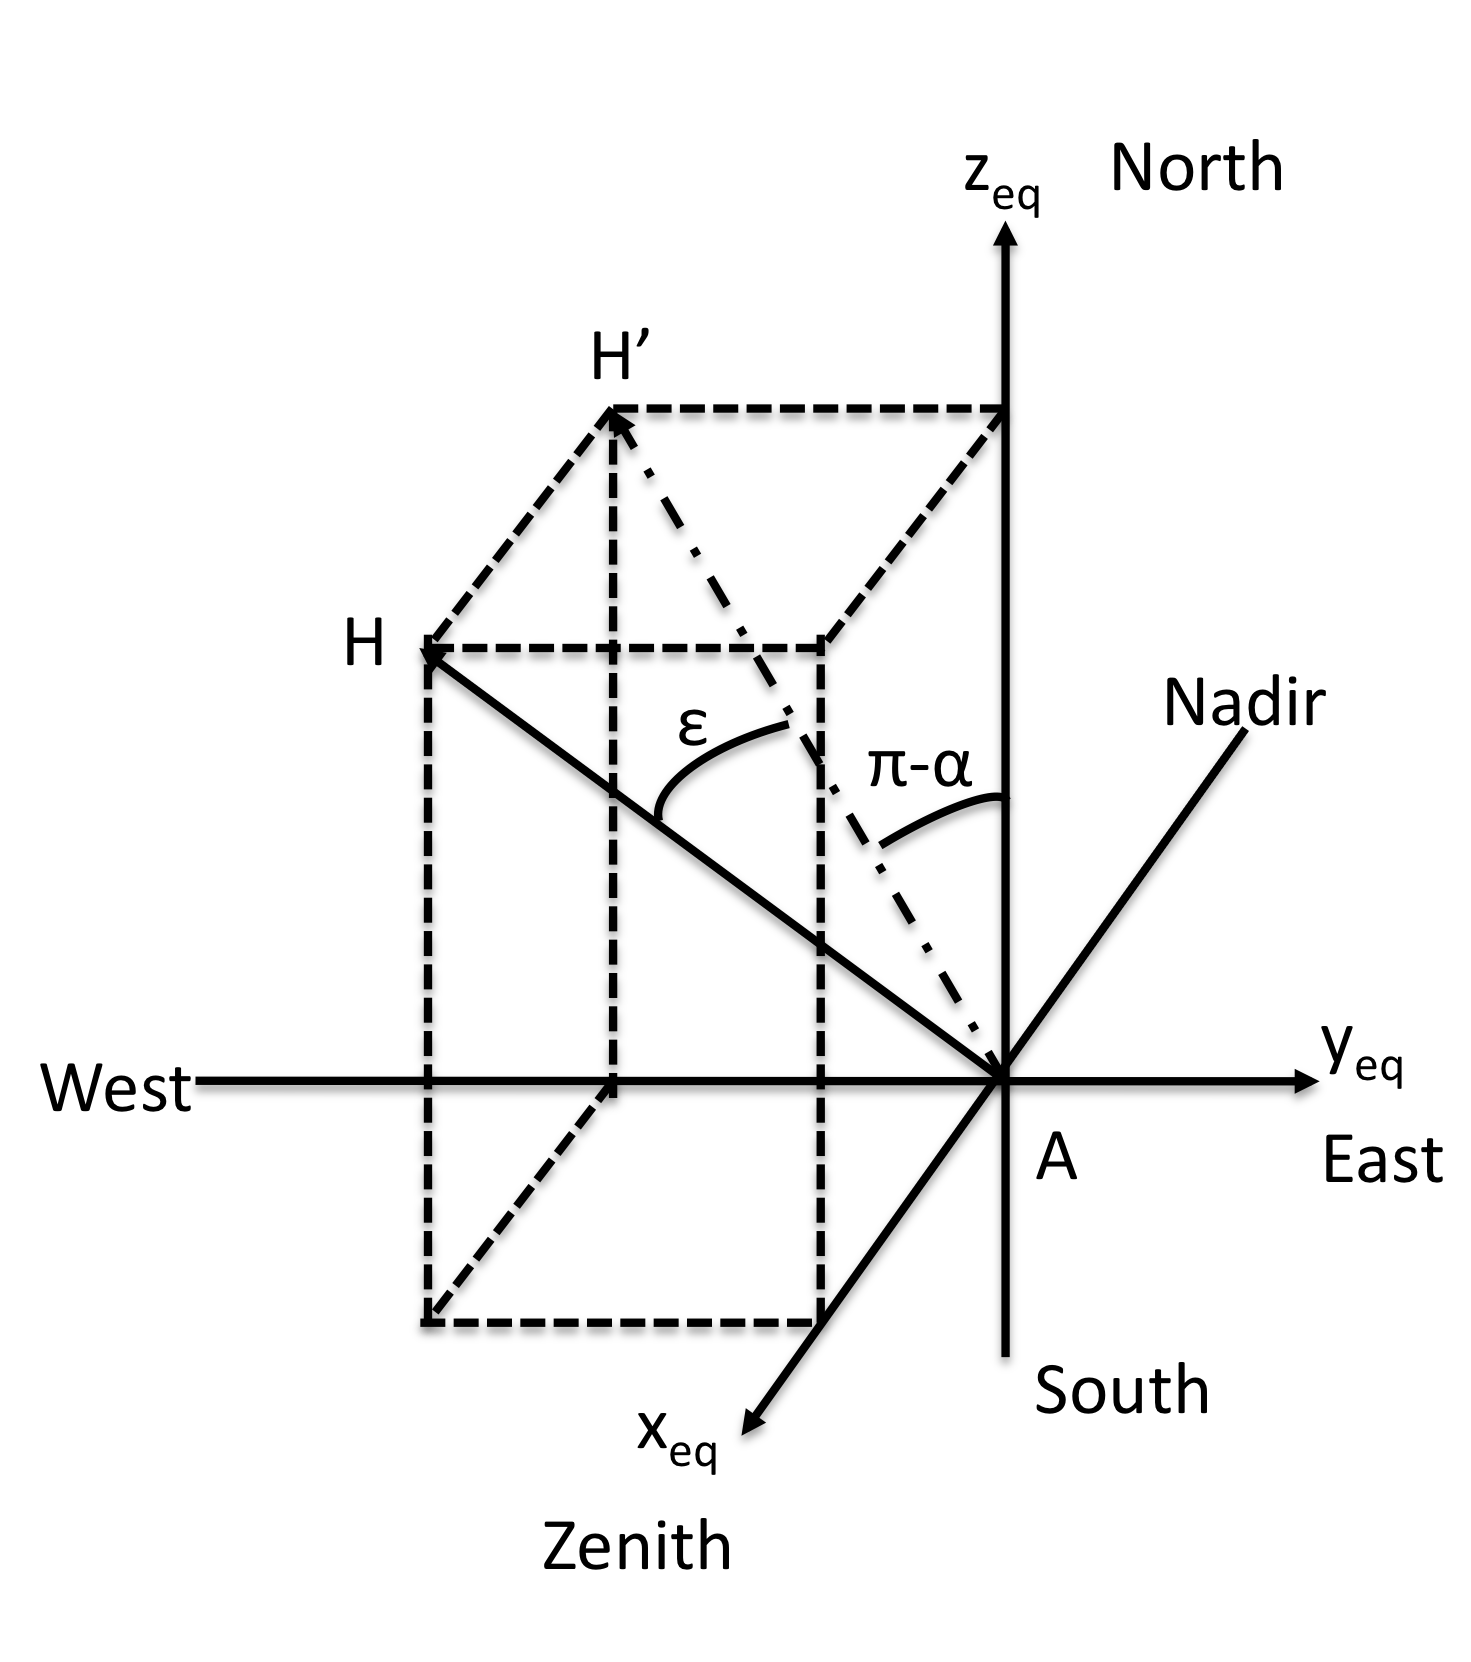
\includegraphics[width=9cm]{figures/geometrie.pdf}
   \caption{Magnification around A of the geometry of the problem when the instrument is at the equator.} 
   \label{geometrie}
   \end{figure}

  \begin{figure}
 \setfigurenum{S4}
   \noindent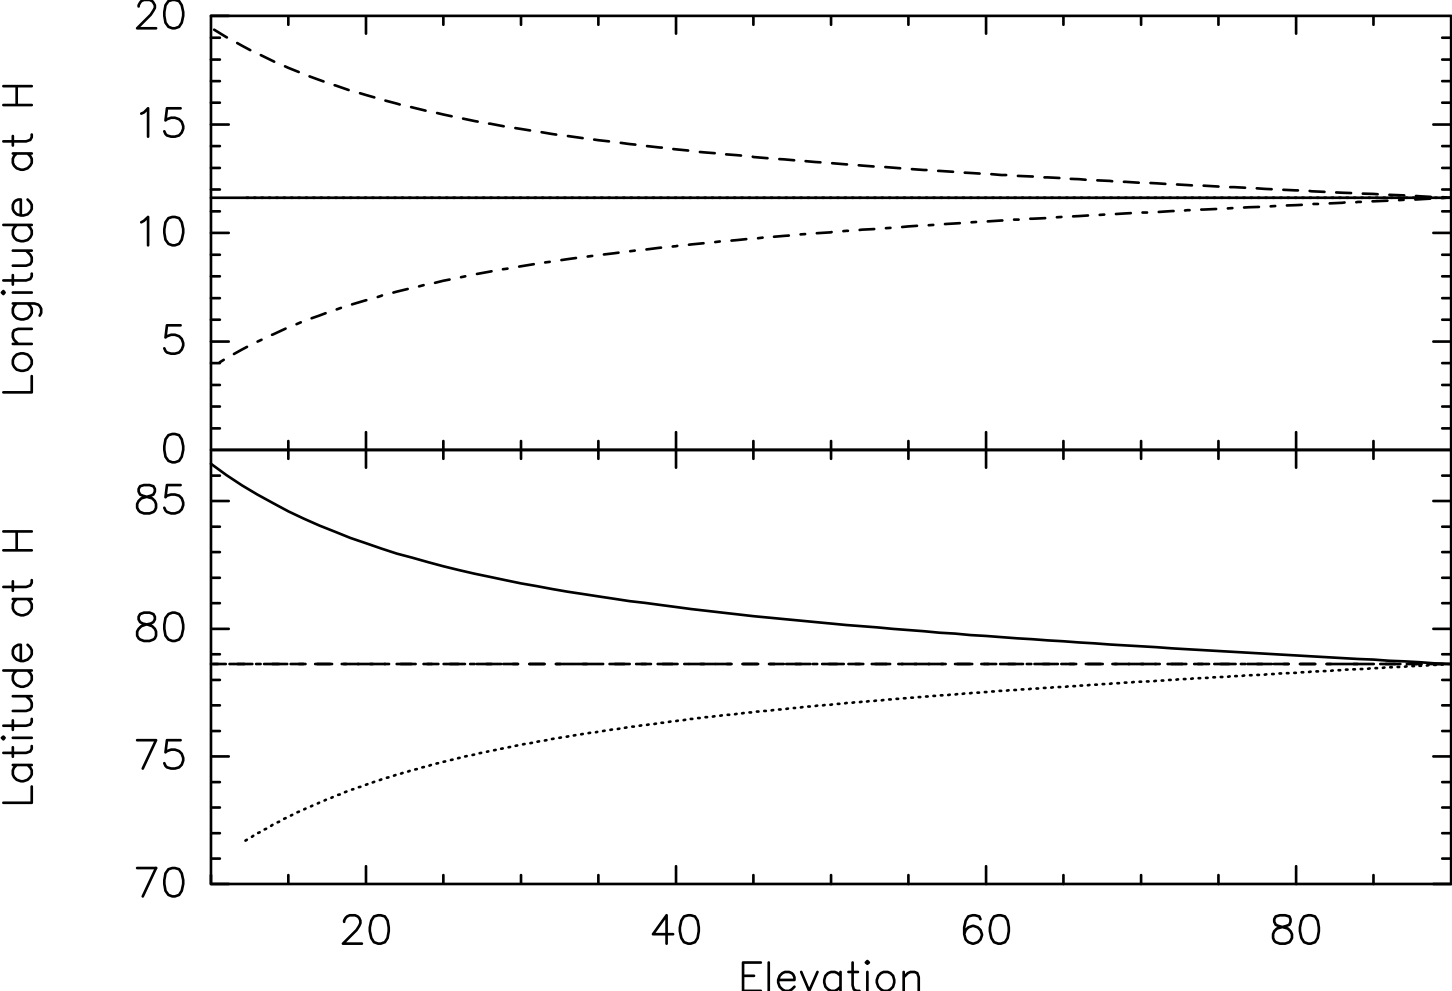
\includegraphics[width=9cm]{figures/angtest.pdf}
   \caption{Latitude (lower panel) and longitude (upper panel) of the point H at 220 km above the ground in the line of sight of the SPP versus its elevation at Svalbard (latitude 78.62 $^\circ$, longitude 11.63 $^\circ$).. The azimuth are north (continuous line), East (dashed line), South (dotted line) and West (dash-dotted line) } 
   \label{angtest}
   \end{figure}

  \begin{figure}
   \setfigurenum{S5}
   \noindent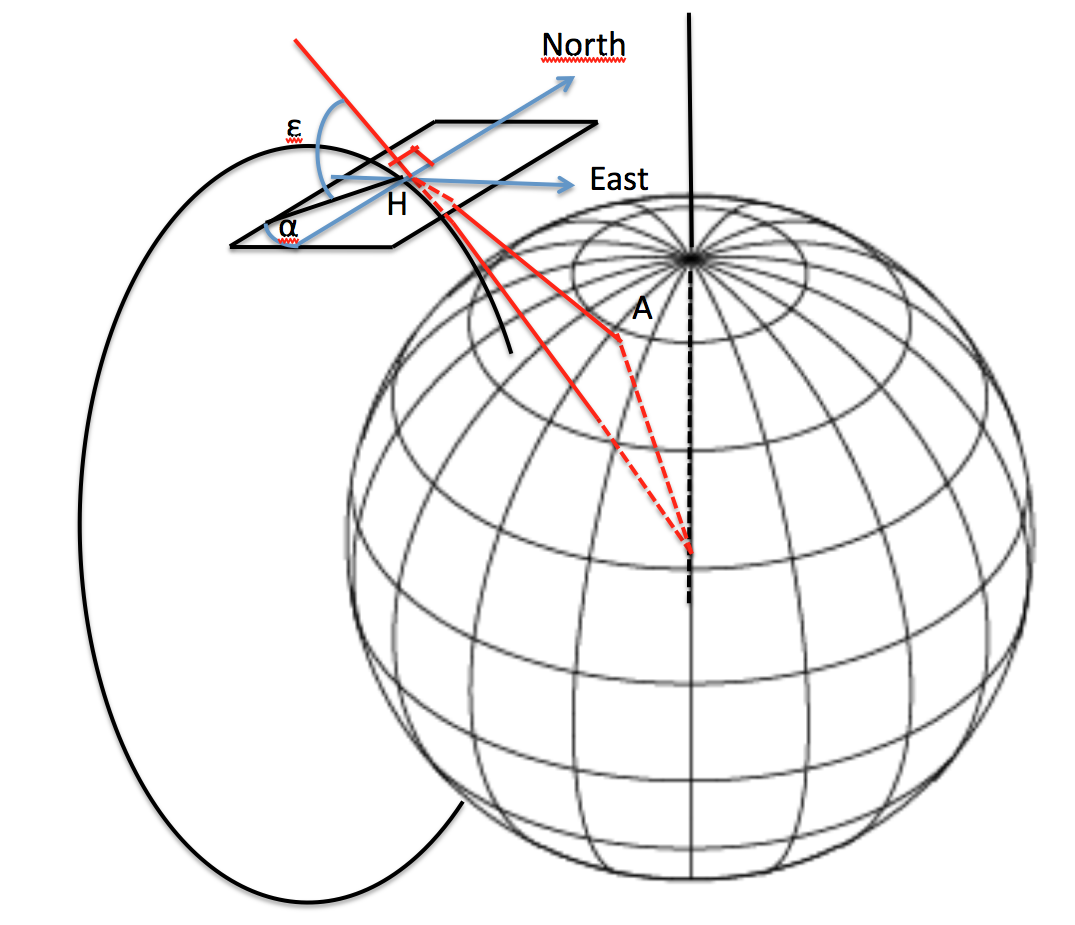
\includegraphics[width=9cm]{figures/ChampMagn.pdf}
   \caption{Geometry of the problem with the magnetic field in H} 
   \label{ChampMagn}
   \end{figure}
   
  \begin{figure}
   \setfigurenum{S6}
   \noindent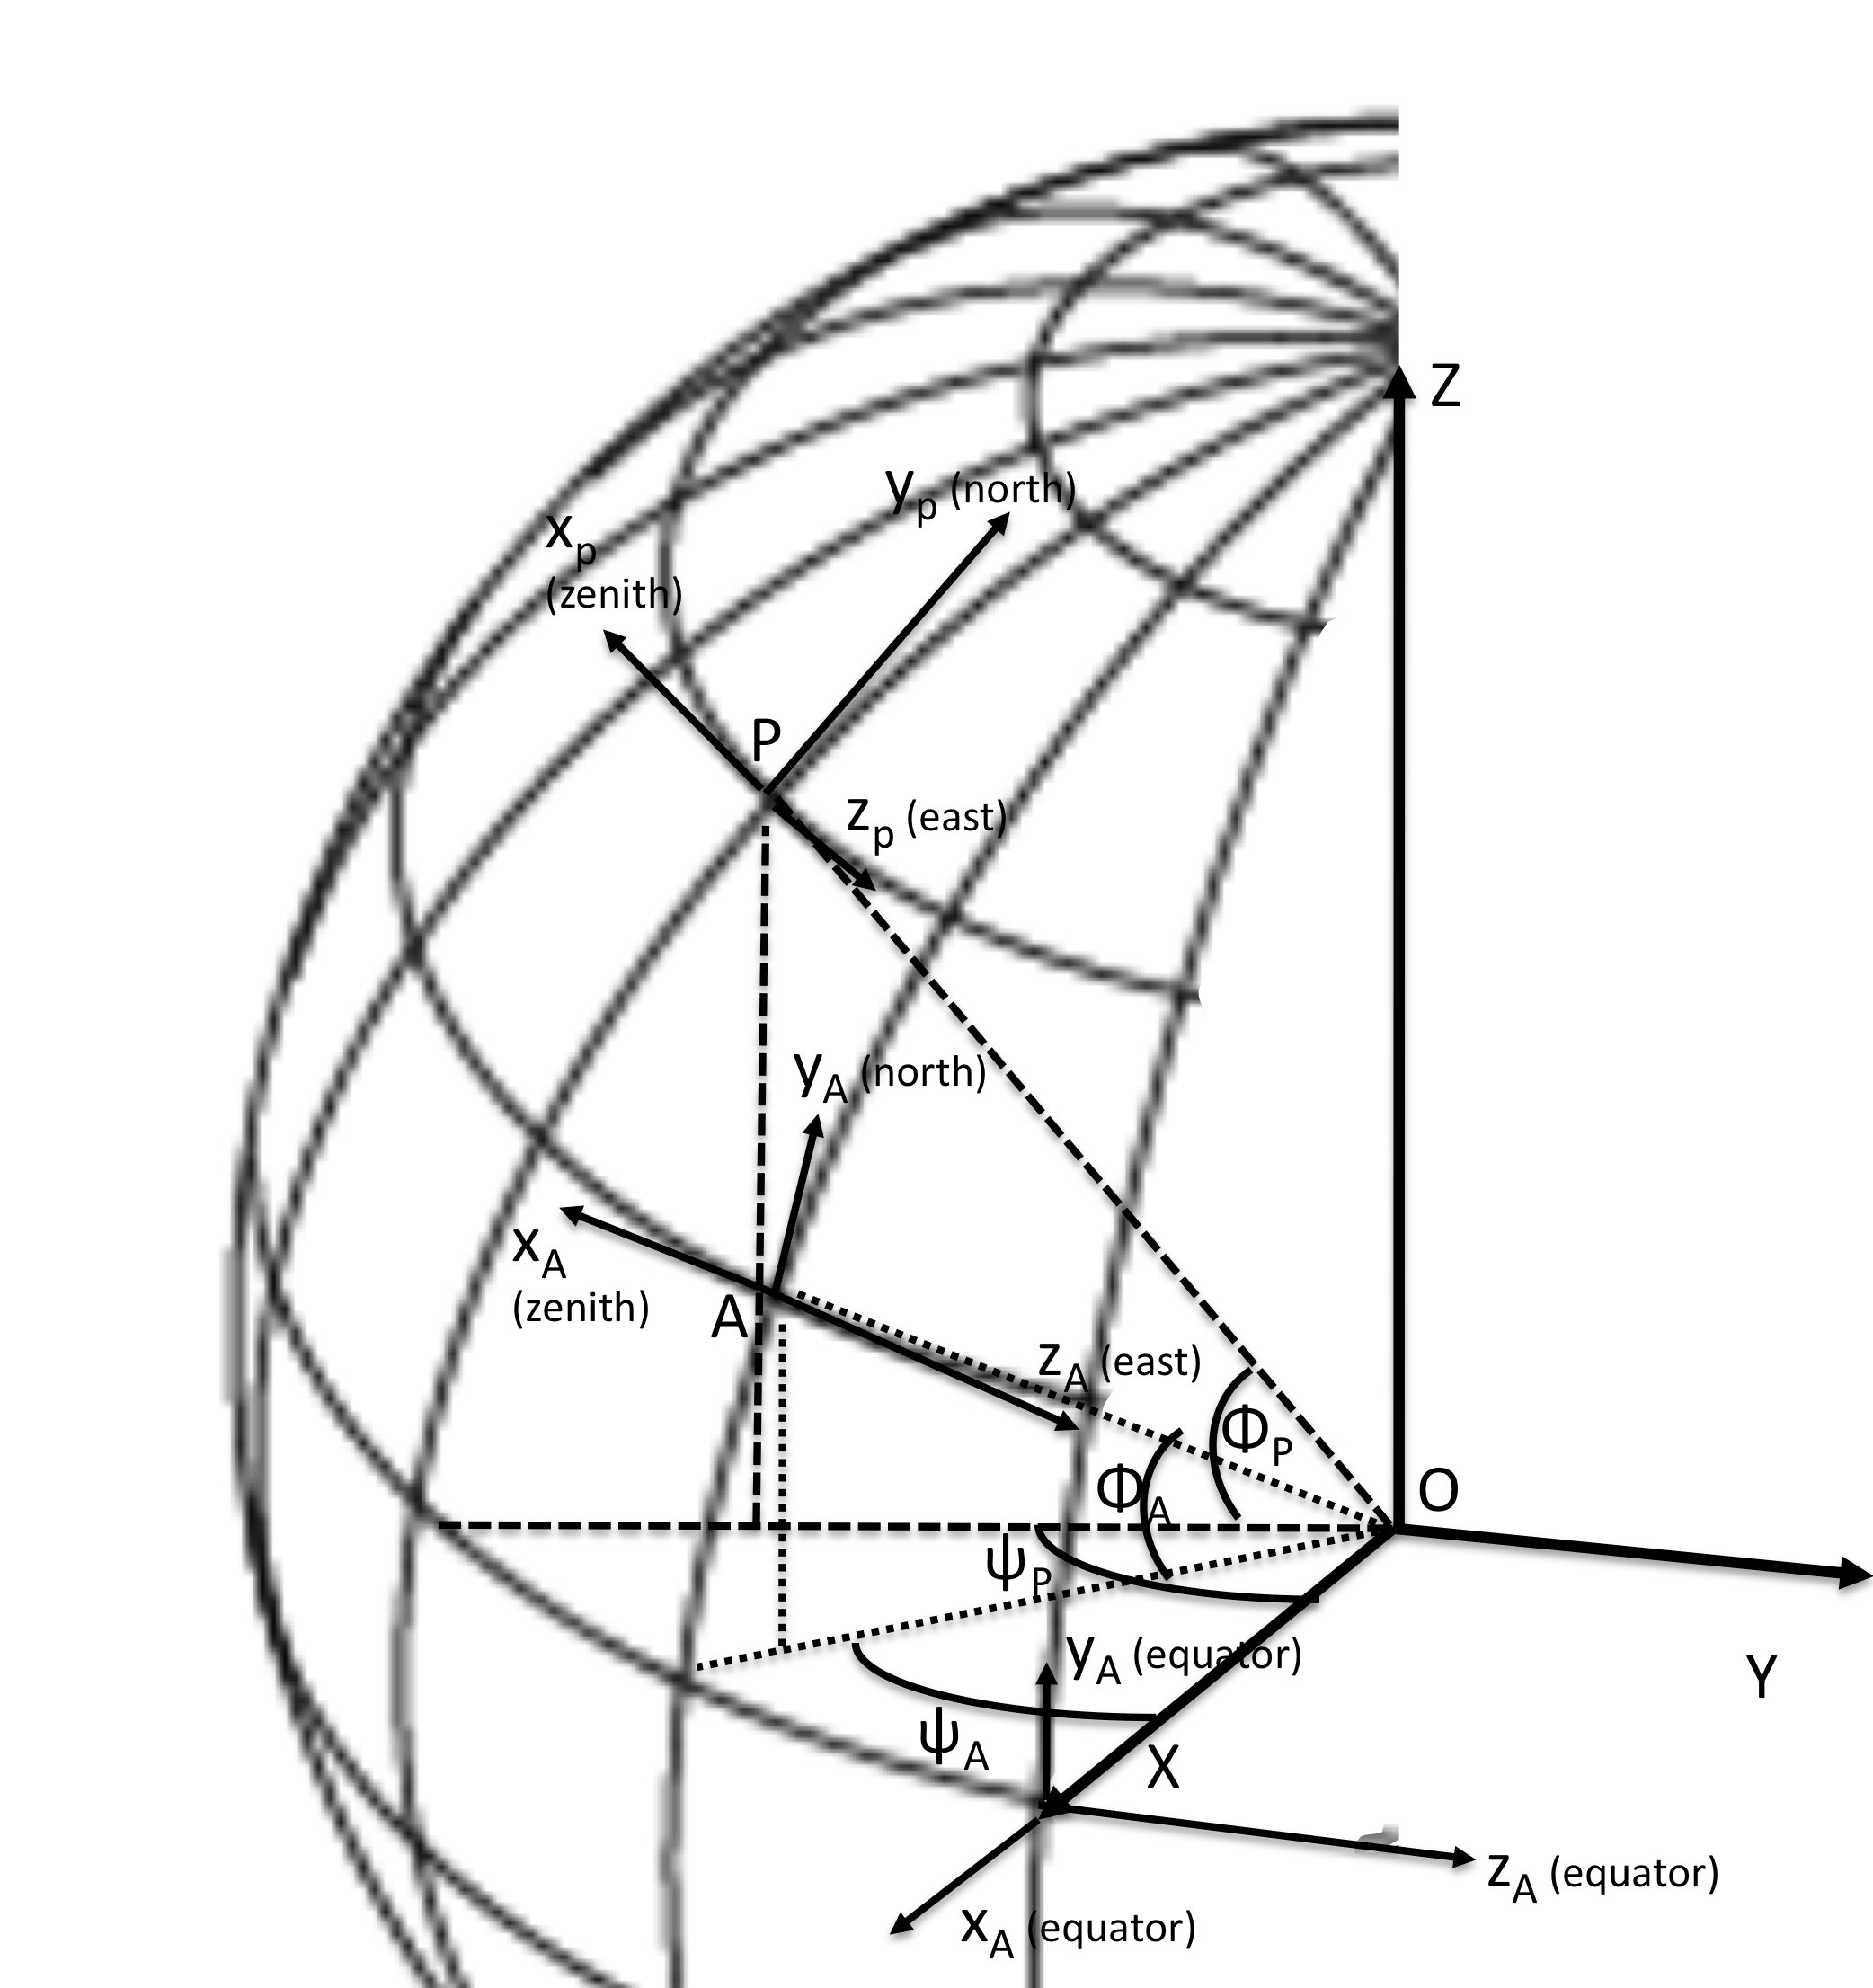
\includegraphics[width=9cm]{figures/Rotation.pdf}
   \caption{The reference frames for the rotations.} 
   \label{rotation}
   \end{figure}
 
   \begin{figure}
   \setfigurenum{S7}
    \noindent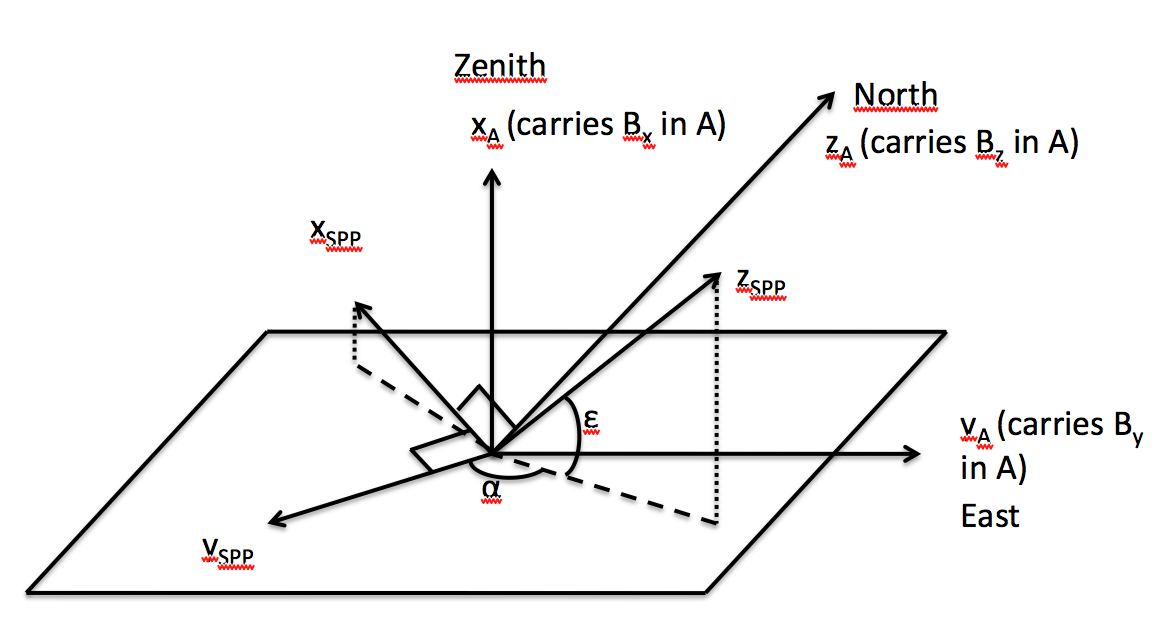
\includegraphics[width=12cm]{figures/lastrot.pdf}
   \caption{The frame of the polarimeter (labelled spp) must be rotated in the frame of A.} 
   \label{lastrot}
   \end{figure}

\begin{figure}
   \setfigurenum{S8}
  \noindent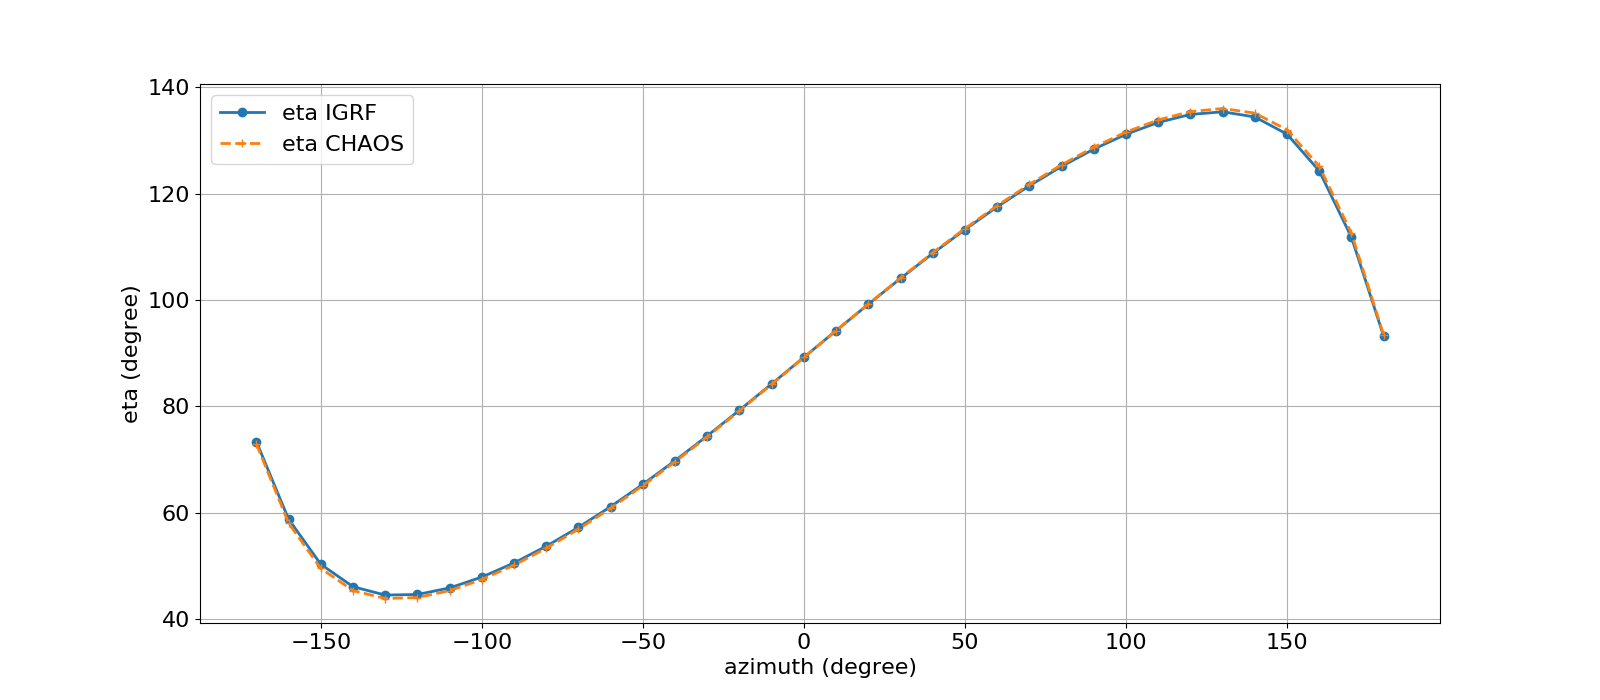
\includegraphics[width=10cm]{figures/eta.pdf}
     \caption{Apparent angle of the magnetic field ($\eta$) projected on the SPP lens (in degrees) as a function of the elevation. The azimuth are north (continuous line), East (dashed line), South (dotted line) and West (dash-dotted line).} 
   \label{fig_eta}
\end{figure}

   \begin{figure}
   \setfigurenum{S9}
    \noindent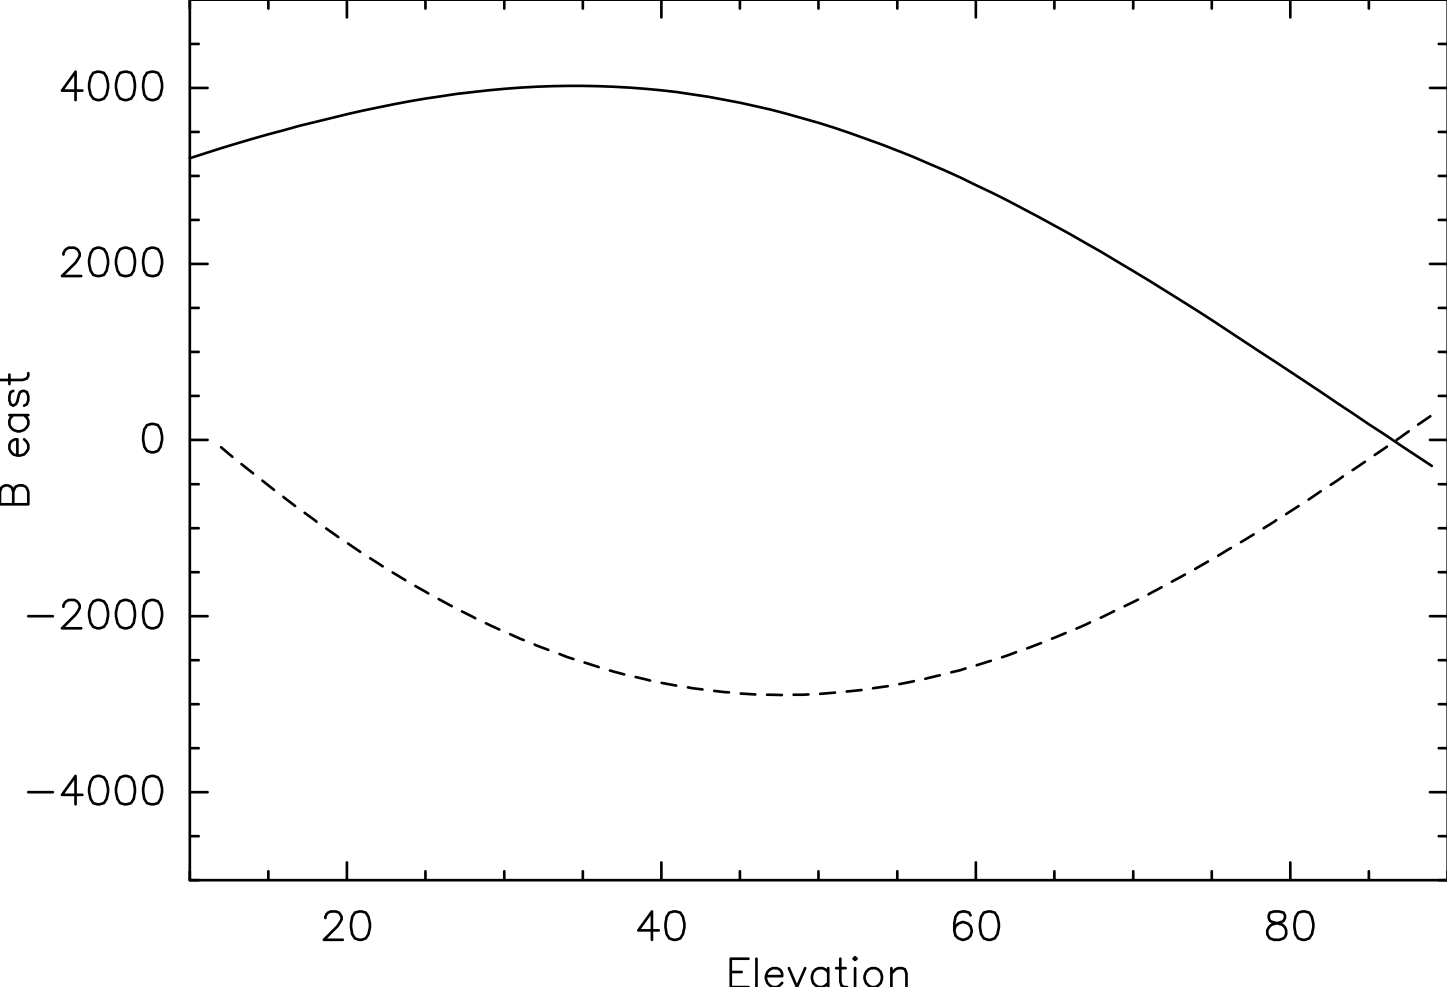
\includegraphics[width=10cm]{figures/wiggle.pdf}
   \caption{Eastward component of the magnetic field projected on the SPP for the north and south azimuths versus the SPP elevation. Continuous line: the SPP pointing North; dashed line: the SPP pointing south.} 
   \label{wriggle}
   \end{figure}

   \begin{figure}
   \setfigurenum{S10}
    \noindent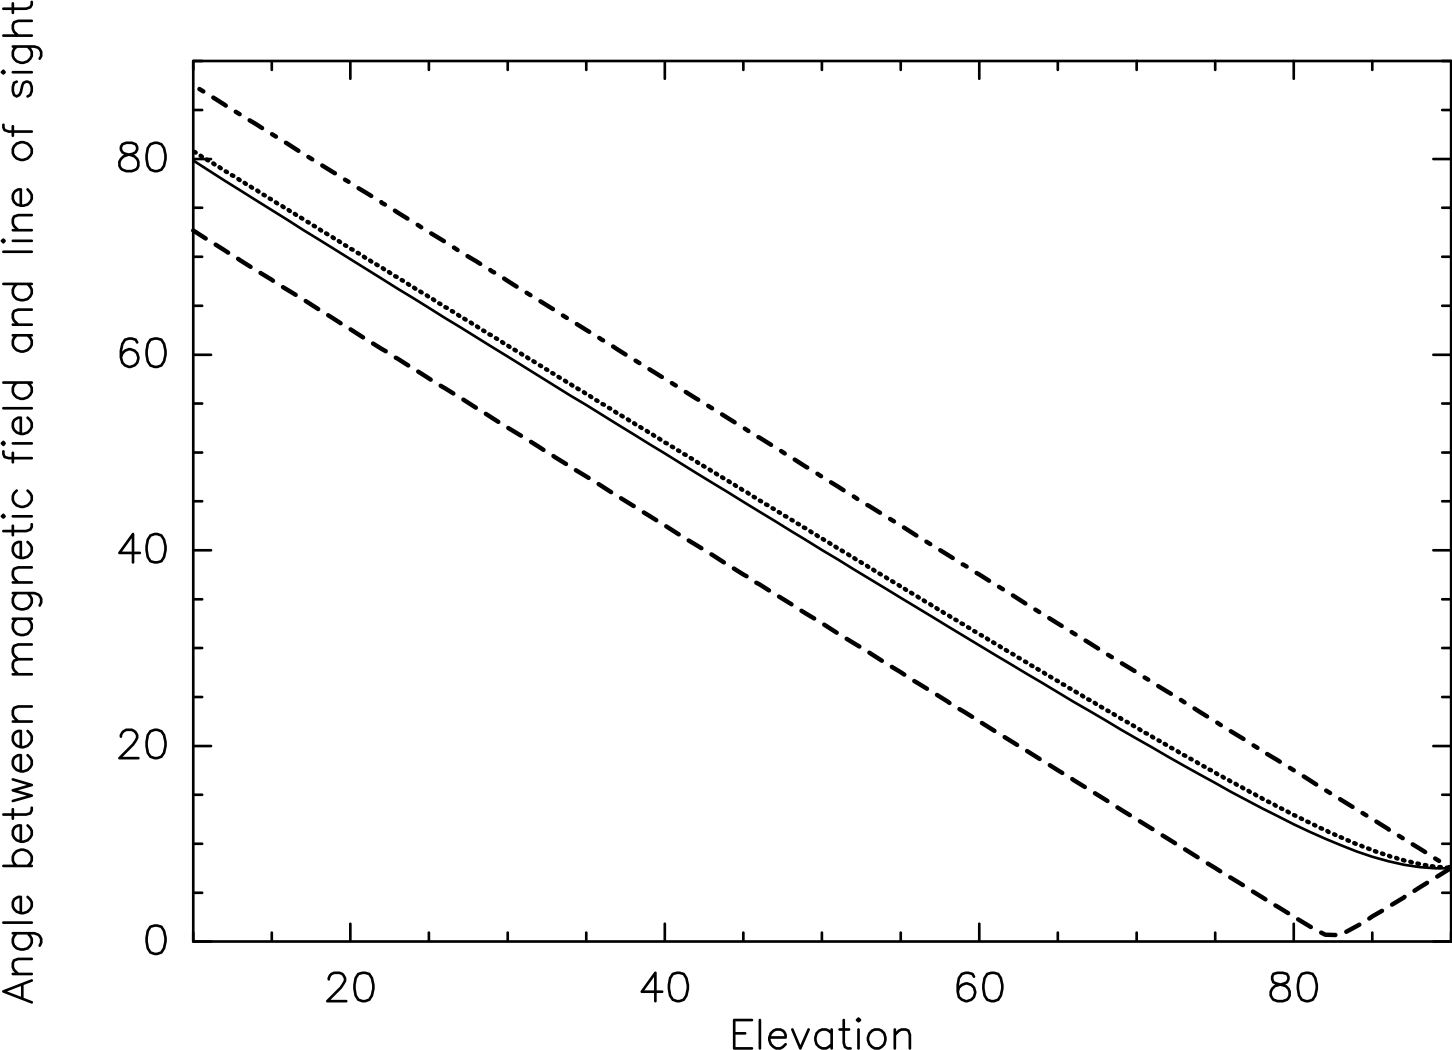
\includegraphics[width=10cm]{figures/b_los_angle2.pdf}
   \caption{Angle between the magnetic field at the emission point H and the SPP line of sight. Continuous line: the SPP pointing North; dashed line: East; dotted line : South; dash-dotted line: West} 
   \label{fig_theta}
   \end{figure}

% ---------------
% EXAMPLE TABLE
%
%\begin{table}
%\settablenum{S1} %%Change number for each table
%\caption{Time of the Transition Between Phase 1 and Phase 2\tablenotemark{a}}
%\centering
%\begin{tabular}{l c}
%\hline
% Run  & Time (min)  \\
%\hline
%  $l1$  & 260   \\
%  $l2$  & 300   \\
%  $l3$  & 340   \\
%  $h1$  & 270   \\
%  $h2$  & 250   \\
%  $h3$  & 380   \\
%  $r1$  & 370   \\
%  $r2$  & 390   \\
%\hline
%\end{tabular}
%\tablenotetext{a}{Footnote text here.}
%\end{table}
% ---------------
%
% EXAMPLE LARGE TABLE (UPLOADED SEPARATELY)
%\begin{table}
%\settablenum{S1} %%Change number for each table
%\caption{Time of the Transition Between Phase 1 and Phase 2\tablenotemark{a}}
%\end{table}


\end{document}

%%%%%%%%%%%%%%%%%%%%%%%%%%%%%%%%%%%%%%%%%%%%%%%%%%%%%%%%%%%%%%%

More Information and Advice:

%% ------------------------------------------------------------------------ %%
%
%  SECTION HEADS
%
%% ------------------------------------------------------------------------ %%

% Capitalize the first letter of each word (except for
% prepositions, conjunctions, and articles that are
% three or fewer letters).

% AGU follows standard outline style; therefore, there cannot be a section 1 without
% a section 2, or a section 2.3.1 without a section 2.3.2.
% Please make sure your section numbers are balanced.
% ---------------
% Level 1 head
%
% Use the \section{} command to identify level 1 heads;
% type the appropriate head wording between the curly
% brackets, as shown below.
%
%An example:
%\section{Level 1 Head: Introduction}
%
% ---------------
% Level 2 head
%
% Use the \section{} command to identify level 2 heads.
%An example:
%\section{Level 2 Head}
%
% ---------------
% Level 3 head
%
% Use the \subsubsection{} command to identify level 3 heads
%An example:
%\subsubsection{Level 3 Head}
%
%---------------
% Level 4 head
%
% Use the \subsubsubsection{} command to identify level 3 heads
% An example:
%\subsubsubsection{Level 4 Head} An example.
%
%% ------------------------------------------------------------------------ %%
%
%  IN-TEXT LISTS
%
%% ------------------------------------------------------------------------ %%
%
% Do not use bulleted lists; enumerated lists are okay.
% \begin{enumerate}
% \item
% \item
% \item
% \end{enumerate}
%
%% ------------------------------------------------------------------------ %%
%
%  EQUATIONS
%
%% ------------------------------------------------------------------------ %%

% Single-line equations are centered.
% Equation arrays will appear left-aligned.

Math coded inside display math mode \[ ...\]
 will not be numbered, e.g.,:
 \[ x^2=y^2 + z^2\]

 Math coded inside \begin{equation} and \end{equation} will
 be automatically numbered, e.g.,:
 \begin{equation}
 x^2=y^2 + z^2
 \end{equation}

% IF YOU HAVE MULTI-LINE EQUATIONS, PLEASE
% BREAK THE EQUATIONS INTO TWO OR MORE LINES
% OF SINGLE COLUMN WIDTH (20 pc, 8.3 cm)
% using double backslashes (\\).

% To create multiline equations, use the
% \begin{eqnarray} and \end{eqnarray} environment
% as demonstrated below.
\begin{eqnarray}
  x_{1} & = & (x - x_{0}) \cos \Theta \nonumber \\
        && + (y - y_{0}) \sin \Theta  \nonumber \\
  y_{1} & = & -(x - x_{0}) \sin \Theta \nonumber \\
        && + (y - y_{0}) \cos \Theta.
\end{eqnarray}

%If you don't want an equation number, use the star form:
%\begin{eqnarray*}...\end{eqnarray*}

% Break each line at a sign of operation
% (+, -, etc.) if possible, with the sign of operation
% on the new line.

% Indent second and subsequent lines to align with
% the first character following the equal sign on the
% first line.

% Use an \hspace{} command to insert horizontal space
% into your equation if necessary. Place an appropriate
% unit of measure between the curly braces, e.g.
% \hspace{1in}; you may have to experiment to achieve
% the correct amount of space.


%% ------------------------------------------------------------------------ %%
%
%  EQUATION NUMBERING: COUNTER
%
%% ------------------------------------------------------------------------ %%

% You may change equation numbering by resetting
% the equation counter or by explicitly numbering
% an equation.

% To explicitly number an equation, type \eqnum{}
% (with the desired number between the brackets)
% after the \begin{equation} or \begin{eqnarray}
% command.  The \eqnum{} command will affect only
% the equation it appears with; LaTeX will number
% any equations appearing later in the manuscript
% according to the equation counter.
%

% If you have a multiline equation that needs only
% one equation number, use a \nonumber command in
% front of the double backslashes (\\) as shown in
% the multiline equation above.

%% ------------------------------------------------------------------------ %%
%
%  SIDEWAYS FIGURE AND TABLE EXAMPLES
%
%% ------------------------------------------------------------------------ %%
%
% For tables and figures, add \usepackage{rotating} to the paper and add the rotating.sty file to the folder.
% AGU prefers the use of {sidewaystable} over {landscapetable} as it causes fewer problems.
%
% \begin{sidewaysfigure}
% \includegraphics[width=20pc]{samplefigure.eps}
% \caption{caption here}
% \label{label_here}
% \end{sidewaysfigure}
%
%
%
% \begin{sidewaystable}
% \caption{}
% \begin{tabular}
% Table layout here.
% \end{tabular}
% \end{sidewaystable}
%
%

